\documentclass[12pt,a4paper,twoside,openany]{book}
\usepackage{textcomp}
\usepackage[T1]{fontenc}
\usepackage[utf8]{inputenc}
\usepackage[italian]{babel}
\usepackage{pdfpages}
\usepackage{graphicx}
\usepackage{rotating}
\usepackage{listings}
\usepackage{caption}
\usepackage{float}
\usepackage{booktabs}
\usepackage{picture}
\usepackage{multirow}
\usepackage{pifont}
\usepackage[hidelinks]{hyperref}
\usepackage{tikz}
\usetikzlibrary{fit,shapes.geometric}

\providecommand*{\cmark}{\ding{51}}
\providecommand*{\xmark}{\ding{55}}

\newcommand\abs[1]{\left|#1\right|}

\newcounter{nodemarkers}
\newcommand\circletext[1]{%
	\tikz[overlay,remember picture] 
	\node (marker-\arabic{nodemarkers}-a) at (0,1.5ex) {};%
	#1%
	\tikz[overlay,remember picture]
	\node (marker-\arabic{nodemarkers}-b) at (0,0){};%
	\tikz[overlay,remember picture,inner sep=2pt]
	\node[draw,ellipse,fit=(marker-\arabic{nodemarkers}-a.center) (marker-\arabic{nodemarkers}-b.center),color=red] {};%
	\stepcounter{nodemarkers}%
}

%codice per mettere logo in sfondo ad ogni pagina
\usepackage{eso-pic}

\AddToShipoutPicture
{
  \put(\LenToUnit{.4\textwidth}, \LenToUnit{.5\textheight}){
\includegraphics{immagini/logo}}%
}

\lstset{basicstyle=\footnotesize\ttfamily\color{black}, language=vhdl, keywordstyle=\color{blue}\bfseries, stringstyle=\color{black}, showstringspaces=false, frame=single, numbers=left, numbersep=5pt, numberstyle=\tiny\color{black}}

\graphicspath{immagini/}
\author{Antonio Riccio - Mat. M63/0605
\and Andrea Scognamiglio - Mat. M63/0598
\and Stefano Sorrentino - Mat. M63/0630}
\title{Elaborato Finale - Task 2 \\ Gruppo 3}

\begin{document}
\frontmatter
\maketitle
\tableofcontents
\setcounter{page}{1}
\mainmatter
\chapter*{Task 2}
Il task prevede la realizzazione di due \textit{IPcore}, ciascuno dei quali andrà a comporre parte dell'architettura di un progetto che prevede la realizzazione di un \textbf{radar bistabile passivo}. 

In questo documento verranno illustrati i concetti fondamentali e le decisioni di progetto che hanno portato alla realizzazione degli artefatti finali, per approfondimenti si rimanda alla documentazione interna e al codice sorgente allegati. 

\chapter{IPcore 1}
Le specifiche per questo componente prescrivono la realizzazione di un \textit{IPcore} che generi campioni di un segnale periodico la cui frequenza e la cui fase possono essere configurati dinamicamente. Le specifiche, inoltre, fissano la frequenza di campionamento del segnale periodico a 20.46 MHz e la possibilità di configurare il numero di campioni da generare in fase di istanziazione del componente. Il campione in uscita deve essere rappresentato su 32 bit di cui 16 bit di parte immaginaria e 16 bit di parte reale.

\begin{figure}[h]
\begin{center}
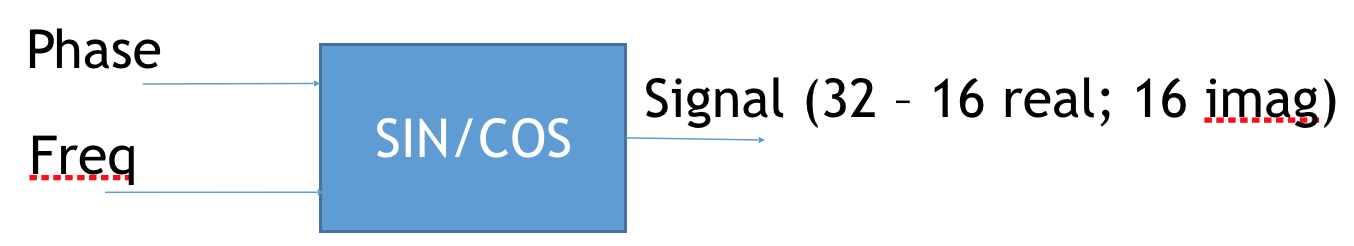
\includegraphics[scale=0.6, keepaspectratio]{immagini/ipcore1_toplevel}
\caption{IPcore 1 ad alto livello}
\label{ipcore1_top}
\end{center}
\end{figure}

\section{Scelta dei componenti}
Per ridurre il tempo di sviluppo dell'\textit{IPcore} sono state effettuate delle ricerche per verificare l'esistenza di blocchi già esistenti. I componenti che più si avvicinavano alle specifiche risultavano essere di \textbf{Xilinx}: in particolare i blocchi \textit{Cordic} e \textit{DDS\_compiler}. Dopo un'attenta lettura dei manuali utente, la scelta è ricaduta sul \textit{DDS\_compiler} poiché il \textit{Cordic} non consentiva di selezionare la frequenza del segnale di uscita ma solo la fase.

Le fasi successive dello sviluppo dell'\textit{IPcore} si sono concentrate sull'adattamento del componente Xilinx in conformità alle specifiche.
\section{Architettura}
L'architettura è formata principalmente dal blocco descritto in precedenza insieme ad altri componenti \textit{riutilizzati} da altri progetti. In particolare, sono stati aggiunti un contatore \textit{modulo-n}, per controllare il numero di campioni da fornire in uscita, ed un'automa a stati finiti, per controllare opportunamente i segnali di controllo del \textit{DDS\_compiler}. L'aggiunta del registro è necessaria poiché l'\textit{IPcore} deve lavorare in un'architettura pipelined. Infine una porta AND viene utilizzata per controllare l'abilitazione del contatore e il caricamento del registro di uscita.  Questi componenti devono essere abilitati solo nel momento in cui il blocco a valle è pronto ad accettare dati, ovvero il segnale \textit{ready\_in} è alto, ed il DDS abbia un valore valido in uscita, ovvero il segnale \textit{valid\_out} è alto. La \figurename~\ref{ipcore1_schemablocchi} mostra come i blocchi sono collegati tra loro.

\begin{figure}
\begin{center}
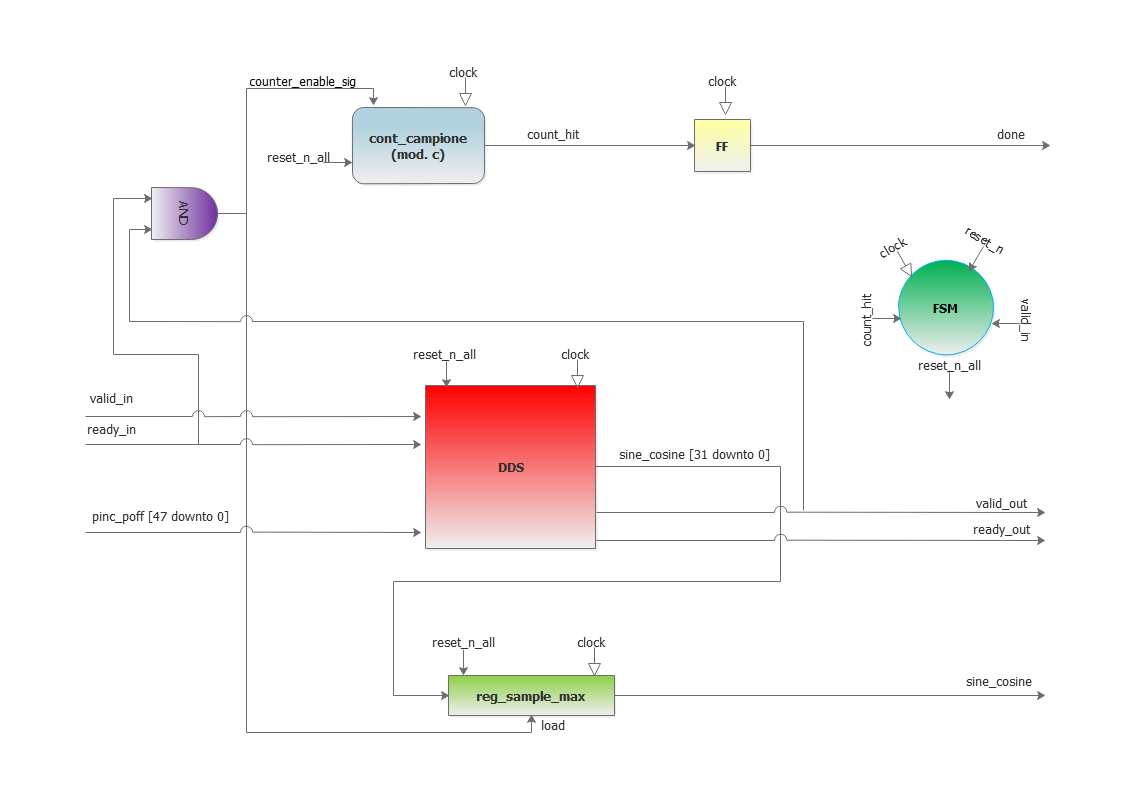
\includegraphics[scale=0.5, keepaspectratio]{immagini/ipcore1_schemablocchi}
\caption{Schema a blocchi di \textit{signal\_generator}}
\label{ipcore1_schemablocchi}
\end{center}
\end{figure}

\clearpage
L'automa a stati finiti, il cui schema è illustrato in \figurename~\ref{ipcore1_fsm}, si occupa di controllare i segnali di controllo del \textit{DDS\_compiler}. Una volta che il segnale \textit{valid\_in} è asserito l'automa resetta il \textit{DDS\_compiler}, abbassando il segnale di \textit{reset} per due periodi di clock, dopodiché si mette in attesa che il contatore abbia terminato il conteggio per poter poi asserire il segnale di \textit{done} e rimettersi in attesa che \textit{valid\_in} sia nuovamente alto.

\begin{figure}
\begin{center}
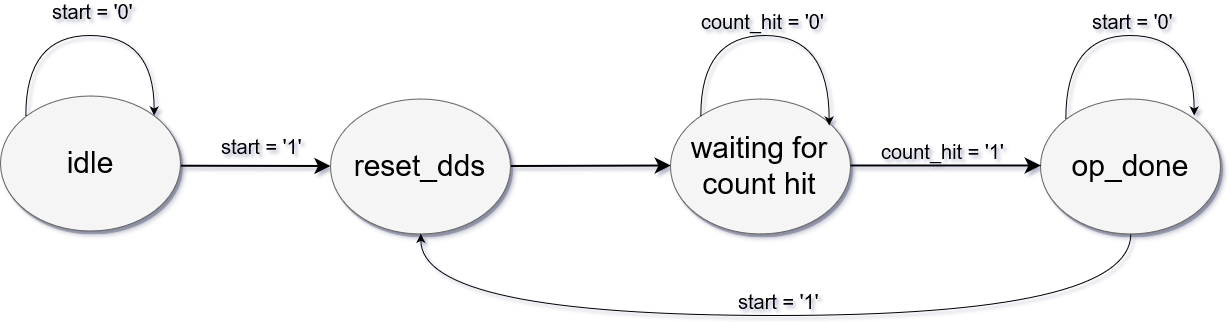
\includegraphics[scale=0.38, keepaspectratio]{immagini/fsm_ipcore1}
\caption{Automa a stati finiti per l'IPcore 1}
\label{ipcore1_fsm}
\end{center}
\end{figure}

\section{Valori di PINC e POFF}
Le specifiche richiedevano di calcolare i valori di spiazzamento di fase e frequenza per ottenere 11 particolari frequenze di uscita che appartenessero all'intervallo compreso tra -3250 e 3000 Hz con salti di 625 Hz. \\
Dal manuale del DDS, la formula per il calcolo della frequenza del segnale in uscita è:
$$
	f_{out} = \frac{f_{clk} \Delta \theta}{2^{B}}
$$

dove:
\begin{itemize}
\item $f_{out}$ è la frequenza del segnale in uscita;
\item $f_{clk}$ è la frequenza di campionamento del segnale (20.46 MHz);
\item $\Delta \theta$ è l'incremento di fase (PINC);
\item B è il numero di bit usati per rappresentare gli spiazzamenti (24 bit).
\end{itemize}

Quindi l'incremento di fase si calcola applicando la formula:
$$
	\Delta \theta = \frac{2^B f_{out}}{f_{clk}} = \frac{2^{24} f_{out}}{20.46 \cdot 10^6}
$$

mentre per le frequenze di uscita \textbf{negative}:
$$
	\Delta \theta = \frac{2^B (f_{clk} + f_{out})}{f_{clk}} = \frac{2^{24} (20.46 \cdot 10^6 + f_{out})}{20.46 \cdot 10^6}
$$

I risultati sono arrotondati all'intero più vicino.

Per quanto riguarda l'offset di fase (POFF), la formula utilizzata è la seguente:
$$
	2 f_{out} p = 2 f_{out} (-0.0005)
$$

Il valore ottenuto deve essere interpretato come un numero a virgola fissa con segno avente un bit di parte intera (il bit di segno).

In base alle formule precedentemente illustrate si ottengono i seguenti valori:\\

\begin{center}
\begin{tabular}{|c|c|c|}
\hline
\textbf{Frequenza} (Hz) & \textbf{PINC} (Hex) & \textbf{POFF} (Hex)\\ 
\hline
-3250								& FFF597					   & 000000						\\
\hline
-2625								& FFF797					   & 000000						\\
\hline
-2000								& FFF998					   & 000FFF						\\
\hline
-1375								& FFFB98					   & FFF000						\\
\hline
-750  								& FFFD99					   & 0F0F0F						\\
\hline
-125									& FFFF99					   & F0F0F0						\\
\hline
500									& 19A						   & FF0000						\\
\hline
1125								& 39B						   & 00FF00						\\
\hline
1750								& 59B						   & 0000DC						\\
\hline
2375								& 79C						   & 003400						\\
\hline
3000								& 99C						   & 220000						\\
\hline
\end{tabular}
\end{center}
\clearpage

\chapter{IPcore 2}
Le specifiche per questo componente prescrivono la realizzazione di un \textit{IPcore} che calcolasse, dato un un insieme di campioni, il massimo valore. I campioni sono espressi come dei valori complessi, formati da parte reale ed immaginaria, i quali devono essere preventivamente elaborati calcolandone il modulo. Il massimo verrà calcolato sui moduli di questi campioni. Il componente deve fornire in uscita il campione (inteso come valore complesso) massimo, oltre alle informazioni relative a spiazzamento nella frequenza doppler, frequenza doppler e satellite ai quali appartiene il campione.

\begin{figure}[hb]
\begin{center}
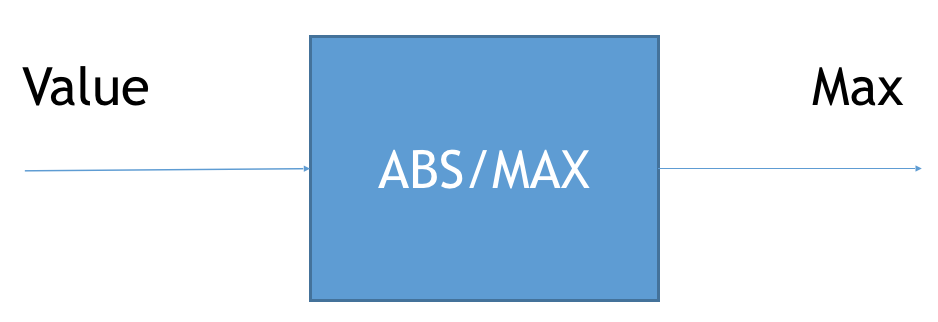
\includegraphics[scale=0.6, keepaspectratio]{immagini/ipcore2_toplevel}
\caption{IPcore 2 ad alto livello}
\label{ipcore2_top}
\end{center}
\end{figure}
\clearpage

\section{Design}
Durante la fase di progettazione si è optato per un approccio realizzativo totalmente \textbf{hardware}. Questa scelta consente di ottenere alta efficienza, in termini temporali, nello svolgimento delle operazioni, che possono essere eseguite anche in parallelo (con i dovuti accorgimenti). 

La scelta di un approccio ibrido o totalmente software non è stata presa in considerazione a causa dell'inefficienza temporale che si può avere introducendo un processore, il quale può non essere ottimizzato per l'applicazione in questione. Sebbene questa motivazione può non sembrare tanto ovvia per il blocco di calcolo del modulo, sicuramente lo è per il blocco che calcola il massimo.

Altra linea guida seguita durante il design è stato il \textbf{riuso}. Qualora possibile, lo sviluppo si è concentrato sul riutilizzo di componenti già presenti e funzionanti, che siano prodotti propri o di terzi.
\section{Architettura}
L'\textit{IPcore} è stato realizzato mediante un approccio \textbf{modulare} per dominare la complessità e facilitare le operazioni di testing.

L'architettura del modulo top-level pertanto è composta da due parti: \textit{complex\_abs} che realizza l'operazione di modulo e \textit{compute\_max} che realizza l'operazione di calcolo del massimo.

\begin{figure}[hb]
\begin{center}
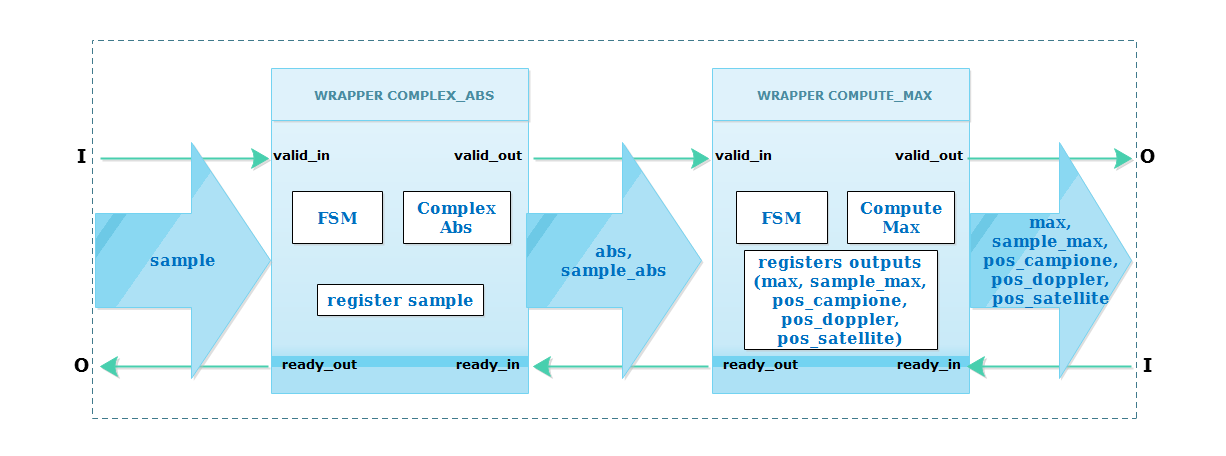
\includegraphics[scale=0.55, keepaspectratio]{immagini/complexmax_schemablocchi}
\caption{Schema a blocchi di \textit{complex\_max}}
\label{complexmax_top}
\end{center}
\end{figure}
\clearpage

\subsection{Calcolo del modulo}
Il componente realizza l'operazione di modulo di un numero complesso secondo la seguente formula:
$$
\abs{z} = \sqrt{x^{2}+y^{2}}
$$
dove \textit{x} e \textit{y} sono, rispettivamente, parte reale e immaginaria del numero complesso \textit{z}.

Siccome le uscite di questo blocco concorrono soltanto al calcolo del massimo e non sono utili ai fini dell'applicazione, si è deciso di escludere il blocco di radice quadrata. Questa operazione è possibile in virtù del fatto che la relazione di \textit{monotonicità} si conserva indipendentemente dall'operazione di radice, pertanto è possibile calcolare il massimo senza necessariamente implementare tutta l'operazione di modulo. Sebbene questa scelta porti a dover gestire un parallelismo di bit superiore (il parallelismo dei dati di uscita è quello dei moltiplicatori e non più della radice), il compromesso diventa accettabile in virtù della disponibilità di area sul silicio.
\subsubsection{Architettura}
L'architettura è composta da due moltiplicatori di \textit{Booth} che calcolano, rispettivamente, il quadrato di parte reale e parte immaginaria del campione in ingresso e da un sommatore \textit{ripple-carry} che somma i risultati dei moltiplicatori.

\begin{figure}[hb]
\begin{center}
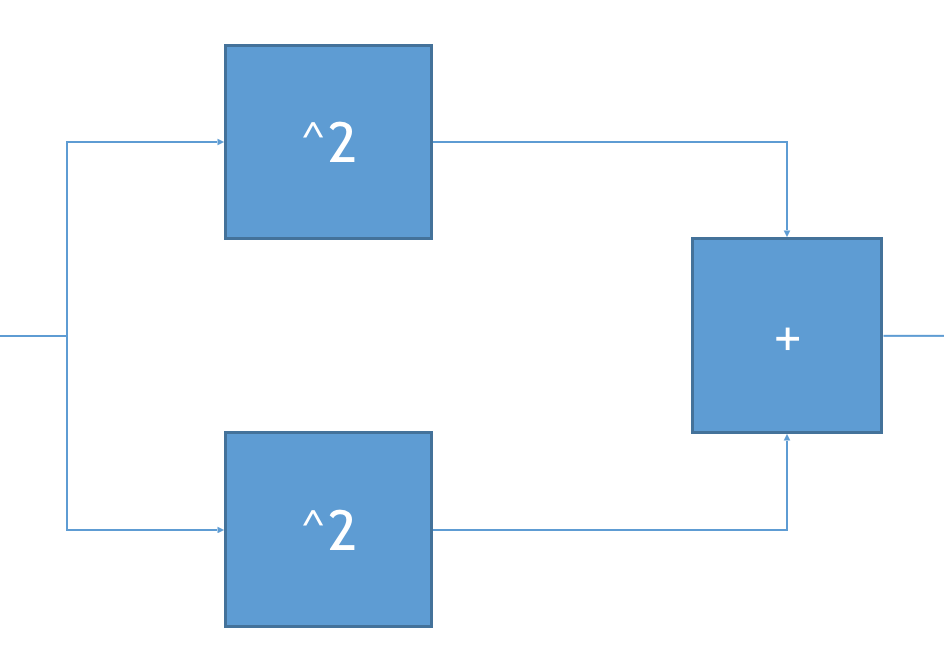
\includegraphics[scale=0.5, keepaspectratio]{immagini/complexabs_schemablocchi}
\caption{Schema a blocchi per \textit{complex\_abs}}
\label{complexabs_schemablocchi}
\end{center}
\end{figure}

Il componente è dotato inoltre di un'unità di controllo alla quale è demandato il pilotaggio dei segnali di abilitazione dei moltiplicatori e del loro reset. 

\begin{figure}
\begin{center}
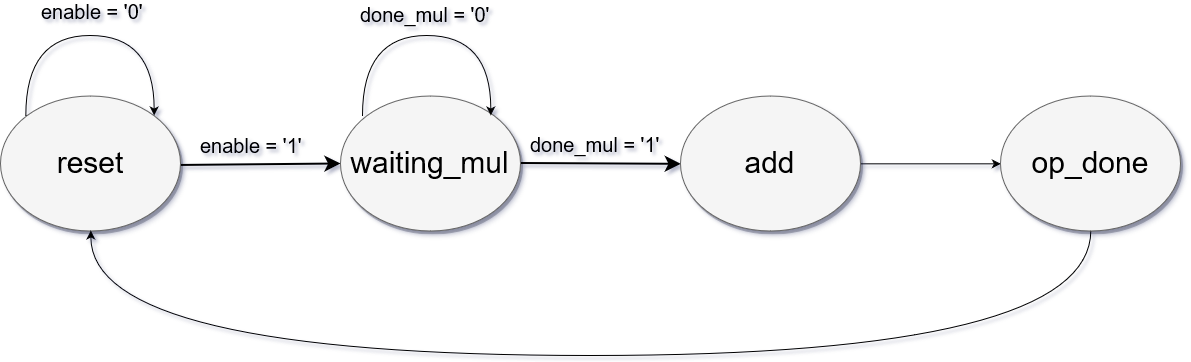
\includegraphics[width=\linewidth, keepaspectratio]{immagini/complexabs_fsm}
\caption{Automa a stati per il blocco \textit{complex\_abs}}
\label{complexabs_fsm}
\end{center}
\end{figure}

Dalla \figurename~\ref{complexabs_fsm}, si può notare la presenza dello stato ADD. Questo stato non comporta nessuna operazione da parte dell'automa se non quella di attendere un periodo di clock necessario al sommatore per completare l'operazione di somma (il sommatore \textit{ripple\_carry} è implementato come macchina combinatoria non pipelined).
\clearpage
\subsection{Calcolo del massimo}
Il componente realizza l'operazione di calcolo del massimo per un insieme di campioni di dimensione $s \cdot d \cdot c$, dove \textit{s} rappresenta il numero di satelliti da analizzare, \textit{d} il numero di intervalli di frequenze doppler per ciascun satellite e \textit{c} rappresenta il numero di campioni per ciascun intervallo doppler. Il massimo viene calcolato sui moduli dei campioni, a loro volta ottenuti dal blocco \textit{complex\_abs}.\\
Per ottimizzare in risorse e tempo lo sviluppo del componente si è incentrato su di una soluzione di calcolo \textbf{dinamico} del massimo: ovvero, ad ogni iterazione, il massimo viene confrontato con il campione in ingresso e aggiornato direttamente. In questo modo si ha la necessità di salvare solo i dati relativi al massimo con conseguente ottimizzazione delle risorse di memoria.

Il componente restituisce in uscita il valore complesso e il modulo del campione massimo oltre alle sue coordinate nell'insieme di campioni, ovvero l'indice di spiazzamento nella frequenza doppler, la frequenza doppler e il satellite ai quali appartiene.

A causa della complessità del componente si è optato per uno sviluppo \textbf{incrementale}: partendo da una descrizione comportamentale, utilizzata per la verifica funzionale, si è poi passati al raffinamento di quest'ultima per individuare i componenti fondamentali e generare un'architettura che descrivesse il blocco come insieme di questi elementi. 

\subsubsection{Architettura behavioral}
Questa architettura è stata sviluppata con l'intento di ottenere velocemente un \textbf{prototipo} del componente, in modo da permettere un testing che consentisse di verificare la correttezza funzionale.

Sostanzialmente il funzionamento del componente è stato sintetizzato a due processi che svolgono compiti ben precisi: uno che elabora il valore dei conteggi e l'altro che effettua i confronti necessari al calcolo del massimo. Per approfondimenti riguardanti le singole fasi dell'algoritmo si rimanda al codice sorgente opportunamente commentato.

\clearpage
\subsubsection{Architettura strutturale}
Essenzialmente l'architettura è caratterizzata da tre \textit{contatori modulo n}, un \textit{comparatore} e cinque \textit{registri}. I contatori servono a realizzare il ciclo di $s \cdot d \cdot c$ iterazioni attraverso una configurazione a cascata. I registri sono necessari per memorizzare le informazioni relative al massimo campione, ovvero il modulo, il valore complesso, lo spiazzamento all'interno della frequenza doppler, l'intervallo doppler e il satellite. Infine il comparatore è necessario per confrontare il campione i-esimo con il massimo. Nella \figurename~\ref{computemax_schema} è possibile osservare come i componenti siano collegati tra loro.

\begin{figure}
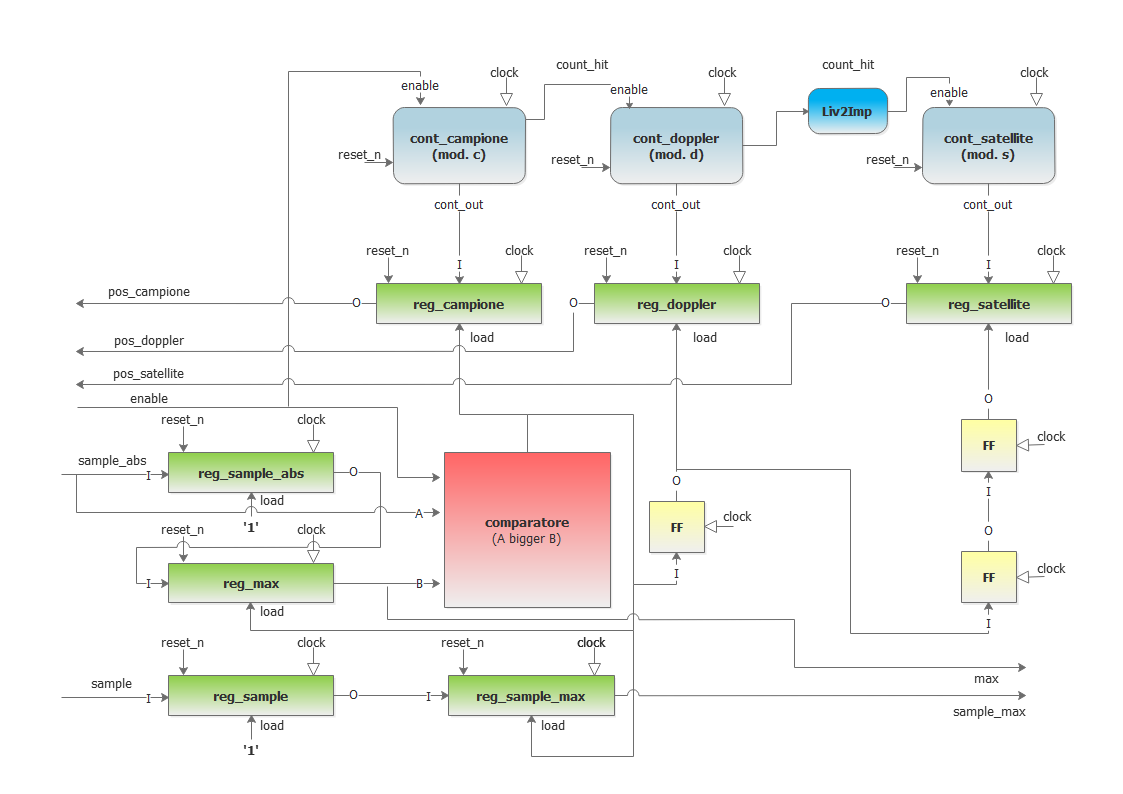
\includegraphics[scale=0.55, keepaspectratio]{immagini/computemax_schemablocchi}
\caption{Architettura strutturale di \textit{compute\_max}}
\label{computemax_schema}
\end{figure}

Ad ogni iterazione, il modulo del campione i-esimo viene confrontato con l'attuale valore massimo mediante il comparatore. Il massimo viene aggiornato solo nel caso in cui il modulo del campione i-esimo sia maggiore dell'attuale modulo massimo. In tal caso, il comparatore asserisce un segnale che va ad abilitare il caricamento di tutti i registri con le informazioni relative al nuovo campione massimo.

Durante lo sviluppo di questa versione sono sorte diverse problematiche, che hanno portato all'introduzione di ulteriori elementi. Questi problemi sono tipici dello sviluppo per componenti, per questo non sono stati riscontrati durante lo sviluppo della versione comportamentale. \\
Due ulteriori registri, \textit{reg\_sample\_abs} e \textit{reg\_sample}, sono stati aggiunti con l'intento di \textbf{ritardare} la variazione del segnale di ingresso. Questo accorgimento è necessario per mantenere stabile il segnale del dato, proveniente dall'esterno, per un tempo tale da consentire ai registri interni di campionare il dato corretto sulla linea di ingresso, nel caso di aggiornamento del massimo.\\
Per un motivo analogo sono stati introdotti dei \textit{flip-flop}, ovvero per ritardare il segnale di caricamento dei registri della doppler e del satellite all'atto dell'aggiornamento del massimo. Questo accorgimento è necessario per consentire ai rispettivi contatori di commutare e consentire ai registri di memorizzare l'indice corretto. Il segnale di caricamento del registro satellite, inoltre, deve tenere in conto di tre ritardi: uno introdotto dal contatore delle doppler, uno introdotto dal componente \textit{livelli2impulsi} e un altro ancora dal contatore dei satelliti. Ovviamente questi segnali potrebbero essere gestiti da un'automa a stati finiti ma si è optato per una soluzione del genere per evitare di complicare il design.\\
Un blocco \textit{livelli2impulsi} è posto tra i contatori delle doppler e dei satelliti per rendere il segnale a livelli \textit{count\_hit} un segnale impulsivo. Questo accorgimento è necessario per evitare che il contatore dei satelliti sia abilitato al conteggio per più di una volta, cosa che potrebbe capitare quando sono terminate le frequenze doppler per un dato satellite (in tal caso il contatore delle doppler avrebbe raggiunto il massimo conteggio e asserirebbe \textit{count\_hit} fino alla prossima abilitazione al conteggio, che avverrebbe solo alla fine della prossima frame).\\
\clearpage
\subsection{Collegamento dei blocchi}
Durante la fase di collegamento dei blocchi appena descritti sono sorti svariati problemi di sincronizzazione derivanti dal fatto che i blocchi avessero tempi di calcolo differenti. 

Una prima soluzione è stata quella di utilizzare frequenze di clock diverse per ciascun blocco, ovvero modellando la frequenza di clock del blocco \textit{compute\_max} con un periodo che tenesse in conto del ritardo del blocco \textit{complex\_abs}, ma questa soluzione è stata abbandonata per la difficoltà di definire in maniera precisa la latenza del primo blocco.

La soluzione adottata, pertanto, è stata quella di utilizzare una comunicazione basata su \textbf{scambio di messaggi}. In pratica, ciascun blocco gestisce una coppia di segnali: \textit{valid\_out} che indica la \textbf{validità} del dato sulla linea di uscita e \textit{ready\_out} che indica la \textbf{disponibilità} del blocco ad accettare dati in ingresso. Oltre a questi due segnali, ciascun blocco riceve in ingresso un'altra coppia di segnali con una semantica simile: \textit{valid\_in}, che indica la validità del dato in ingresso al blocco (asserito dal blocco a monte) e \textit{ready\_in}, che indica la disponibilità del componente a valle di accettare dati. \\
Come si può osservare dalla \figurename~\ref{wrapperabs_fsm}, ogni qualvolta un blocco è pronto ad accettare dati in ingresso deve asserire \textit{ready\_out} e attendere che \textit{valid\_in} sia asserito dal blocco a monte. Una volta che \textit{valid\_in} diventa alto, il blocco può procedere all'elaborazione e asserire \textit{valid\_out}, quando l'elaborazione termina, per segnalare la presenza di dati validi sulla linea di uscita. Se il blocco a valle non è pronto ad accettare dati, il blocco dovrà attendere che il segnale \textit{ready\_in} sia alto prima di procedere al calcolo successivo.

\begin{figure}
\begin{center}
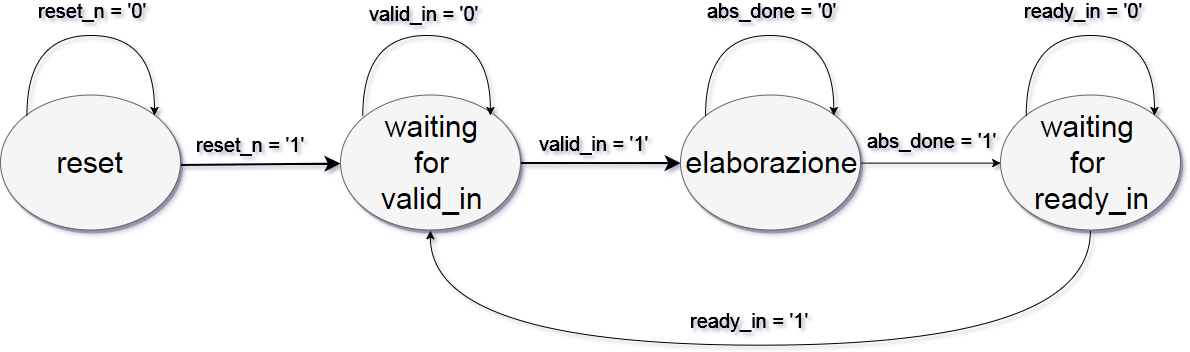
\includegraphics[scale=0.35, keepaspectratio]{immagini/fsm_wrapper_abs}
\caption{Protocollo di comunicazione}
\label{wrapperabs_fsm}
\end{center}
\end{figure}

\clearpage
\begin{figure}
\begin{center}
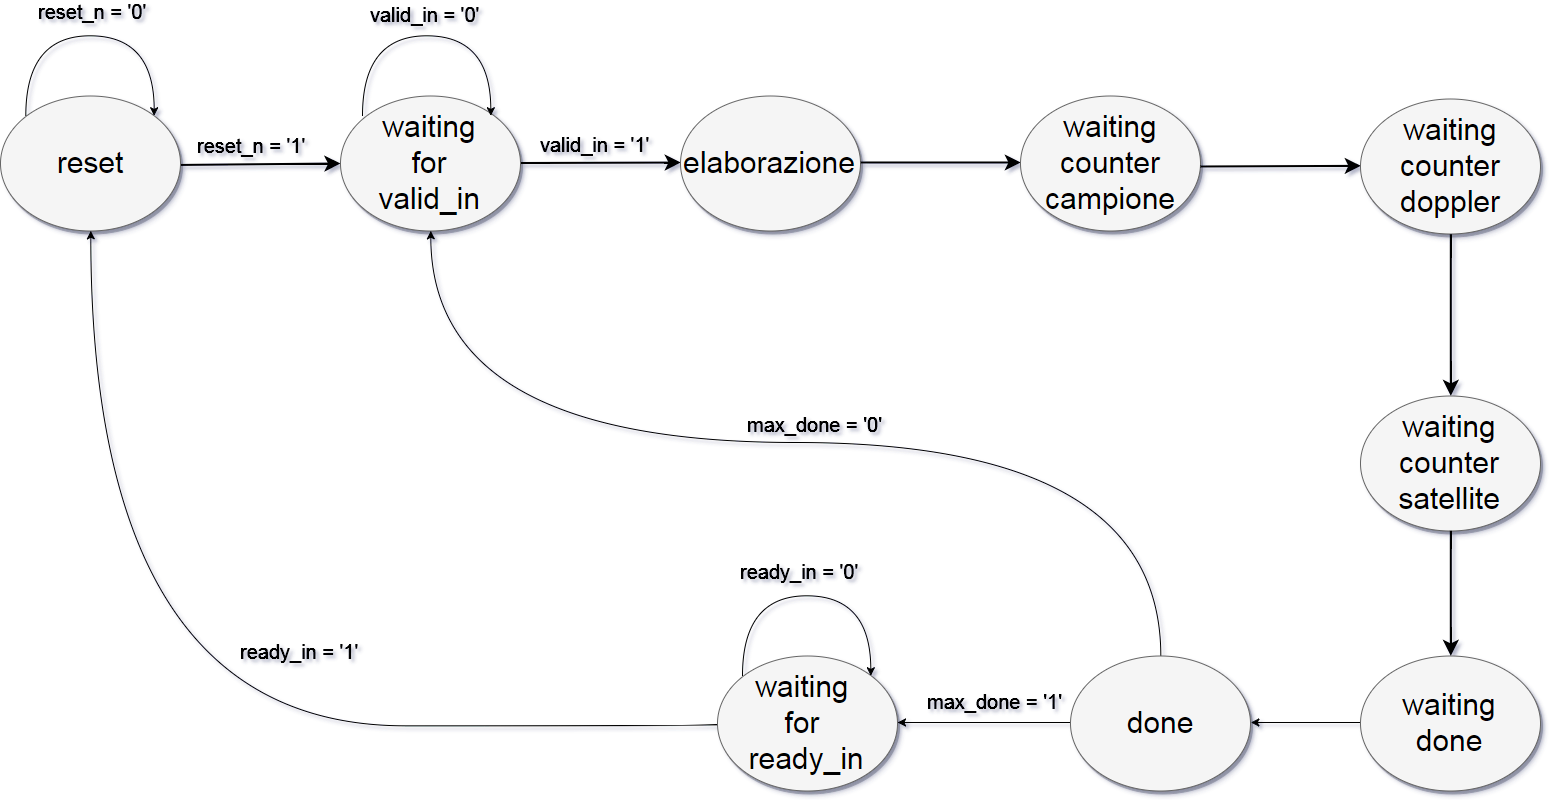
\includegraphics[scale=0.28, keepaspectratio]{immagini/fsm_wrapper_max}
\caption{Protocollo di comunicazione per \textit{compute\_max}}
\label{wrappermax_fsm}
\end{center}
\end{figure}

La \figurename~\ref{wrappermax_fsm} mostra l'automa riguardante \textit{compute\_max}. Esso presenta una piccola variazione rispetto a quello per \textit{complex\_abs} ovvero l'introduzione di alcuni stati di attesa che sono necessari per consentire l'aggiornamento corretto di tutte le uscite.

Per ridurre al minimo le modifiche al codice dei componenti, già testato e funzionante, si è optato di aggiungere le funzionalità di comunicazione attraverso l'utilizzo di \textit{wrapper}. Ogni \textit{wrapper} contiene il relativo componente e l'automa a stati che implementa il protocollo di comunicazione, oltre ad alcuni registri che sono necessari per memorizzare il risultato dell'elaborazione.

L'aggiunta delle funzionalità di comunicazione e dunque della eventualità che il blocco possa fermarsi in attesa di dati validi in ingresso ha portato a delle leggere modifiche all'architettura di \textit{complex\_max}.\\
Le modiche hanno riguardato la rimozione dei registri usati per ritardare gli ingressi, \textit{reg\_sample\_abs} e \textit{reg\_sample\_max}, poiché il ritardo necessario a mantenere stabili gli ingressi viene fornito direttamente dall'automa nel wrapper. Inoltre, l'ingresso di abilitazione al conteggio per il contatore dei campioni viene passato all'esterno poiché è sempre l'automa del wrapper a determinarne l'incremento quando necessario. Infine, viene aggiunto un altro blocco \textit{livelli2impulsi}, tra il contatore dei campioni e quello delle doppler, proprio perché il contatore dei campioni non è sempre abilitato e quindi potrebbe generare un segnale di \textit{count\_hit} che permane alto fintantoché non viene nuovamente abilitato al conteggio. L'introduzione di quest'ultimo blocco provoca un'ulteriore latenza che deve essere compensata da un ulteriore \textit{flip-flop} per il segnale di caricamento del registro della doppler. La \figurename~\ref{computemax_schema2} illustra come cambia l'architettura per il blocco \textit{compute\_max} in seguito alle osservazioni precedenti.

\begin{figure}
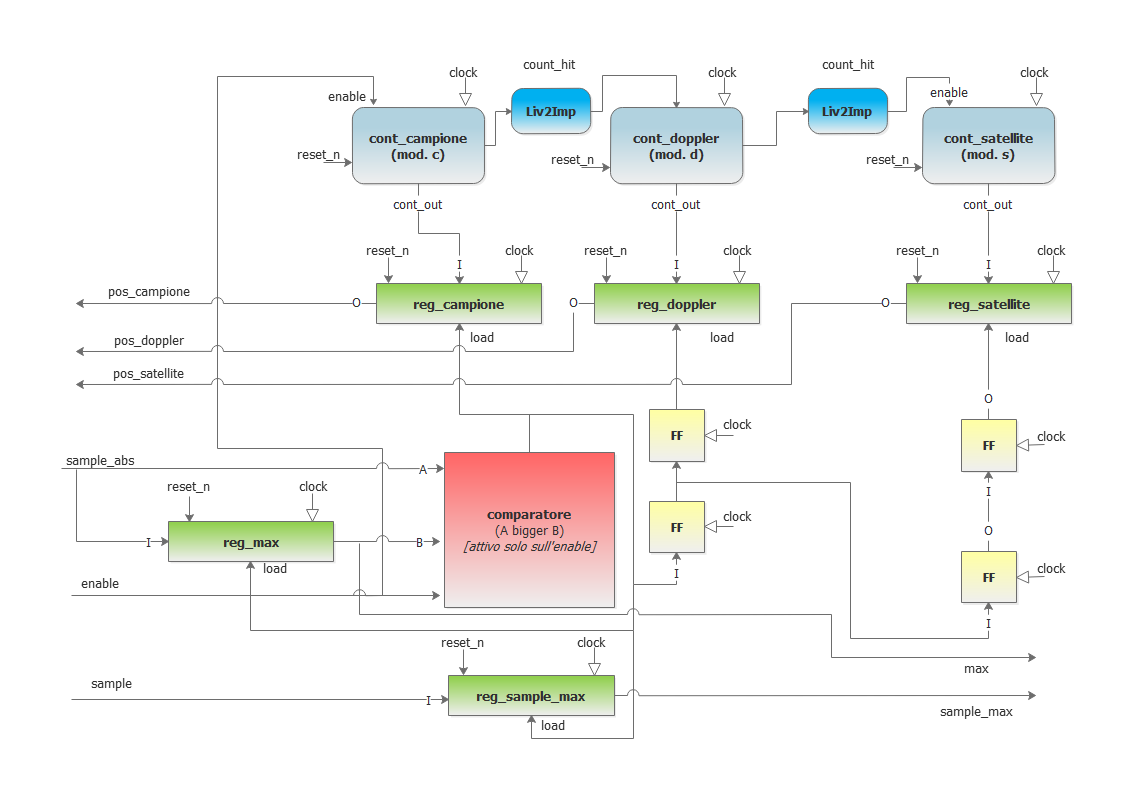
\includegraphics[scale=0.55, keepaspectratio]{immagini/computemax_schemablocchi2}
\caption{Architettura strutturale (rivista) di \textit{compute\_max}}
\label{computemax_schema2}
\end{figure}
\end{document}
